\chapter{仿真实验}
在上一节中,我们基于双反馈Thompson Sampling算法开发了5个针对周期信道的优化算法(下面统称为TS算法)。在下面的仿真实验中,我们假设不知道信道的周期。如果知道了信道的周期,那么显然我们不再需要这些改进的双反馈TS算法。因为我们可以在每次周期改变的时候切换到上一次周期积累的数据。另外在考虑如何设定传输概率组数时,我们选择设定两组数据,根据我们的实验数据,两组数据就能大致展示出实验结果,且实验结果与10组、25组等更多的组也大致相同。在模拟中,我们将时间范围设置为$10^4$个时隙,并运行$5000$个实验以确保平均遗憾是足够精确的。表 \ref{tabA1} 表示仿真实验参数设置。
\begin{table}[h]
	\centering
	\caption{仿真实验参数设置}		
	\label{tabA1}
	\begin{tabular}{c|c|c|c|c|c}
		\toprule[2pt]
		& Rate1 & Rate2 & Rate3 & Rate4 & Rate5 \\
		\midrule[2pt]
		传输速率$r_{n}$	& 2	& 3	& 5 & 7 & 9 \\
		\hline                                        %细横线
		预测概率$\alpha_{n}$ & 0.1 & 0.3 & 0.6 & 0.7 & 0.9 \\
		\hline                                         %细横线
		传输概率$\beta_{n}^{(1)}$ & 0.9 & 0.8 & 0.65 & 0.63 & 0.1 \\
		\hline
		平均吞吐量$1$ & 0.18 & 0.72 & 1.95 & 3.087 & 0.81 \\                                      %细横线
		\hline   
		传输概率$\beta_{n}^{(2)}$ & 0.99 & 0.85 & 0.75 & 0.15 & 0.01 \\
		
		\hline
		平均吞吐量$2$ & 0.198 & 0.765 & 2.25 & 0.735 & 0.081 \\
		\bottomrule[2pt]
	\end{tabular}
\end{table}
\section{置零时机对TS算法的影响}
在这小节,我们研究置零时机对TS算法的影响。我们的实验是基于并不知道信道容量周期的条件进行的,因此很难把握在周期变化的时候置零,因此我们探索置零时机对TS算法的影响。下图中的置零偏差是指置零的时机与周期长度之比。图 \ref{fig置零} 显示出了结果。可以看出置零时机对置零结果影响重大.只有准确的在周期发生改变时进行置零是最好的,其他情况下的结果都是非常差的。但是现实中我们难以把握这个时机,因此置零TS算法的实际应用效果应该没有那么好。
\begin{figure}[h]
	\centering
	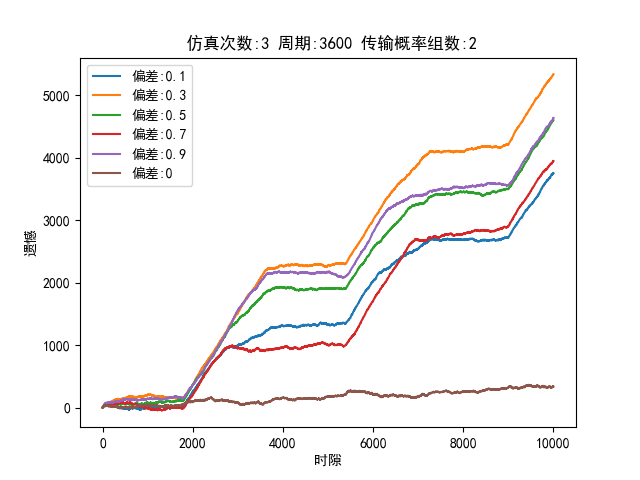
\includegraphics[width=0.8\textwidth]{figure/置零.png}
	\caption{置零时机对TS算法的影响} 
	\label{fig置零}
\end{figure}


\section{总体比较}
在本小节中,我们将比较七个算法的遗憾性能。这七个算法分别是单反馈的Thompson Sampling算法、两层反馈的Thompson Sampling算法、周期性重置Thompson Sampling算法、基于折扣的Thompson Sampling算法、基于滑动窗口的Thompson Sampling算法、基于增加次数的滑动窗口Thompson Sampling算法和基于折扣、增加次数和滑动窗口的Thompson Sampling算法。图 \ref{fig总}可以看出经过改进的TS算法表现都非常优秀。
\begin{figure}[h]
	\centering
	\includegraphics[width=0.8\textwidth]{figure/总.png}
	\caption{七个算法小周期的效果比较图} 
	\label{fig总}
\end{figure}


\section{窗口容量对TS算法的影响}
在这小节,我们选定基于滑动窗口的TS算法来研究窗口容量对TS算法的影响。窗口容量的单位设定为时间,即窗口容量表示能存储多少时隙的结果。我们设定了8个窗口容量值,100、250、300、500、800、1000和2000。图 \ref{fig窗口}显示窗口容量值处于250-500的表现都非常好。
\begin{figure}[h]
	\centering
	\includegraphics[width=0.8\textwidth]{figure/窗口.png}
	\caption{窗口容量对TS算法的影响}
	\label{fig窗口}
\end{figure}

\section{折扣系数对TS算法的影响}
在这小节,我们选定基于折扣的Thompson Sampling算法来研究折扣系数对TS算法的影响。我们设定了5个折扣系数值,分别为0.1、0.5、0.8、0.9、0.95和1。令人惊讶,图 \ref{fig系数}显示出折扣系数为1的算法表现更佳。折扣系数对TS算法的影响和窗口容量关系比较大,很可能是测试的这个窗口容量条件导致的结果。
\begin{figure}[h]
	\centering
	\includegraphics[width=0.8\textwidth]{figure/系数.png}
	\caption{折扣系数对TS算法的影响}
	\label{fig系数}
\end{figure}

\section{增加失败次数对TS算法的影响}
在这小节,我们选定基于折扣的Thompson Sampling算法来研究折扣系数对TS算法的影响。我们设定了5个折扣系数值,分别为0.1、0.5、0.8、0.9、0.95和1。令人惊讶,图 \ref{fig失败}显示出失败次数对结果没有影响。这说明在某一个手臂失败的时候它被选择的次数并没有超过窗口。
\begin{figure}[h]
	\centering
	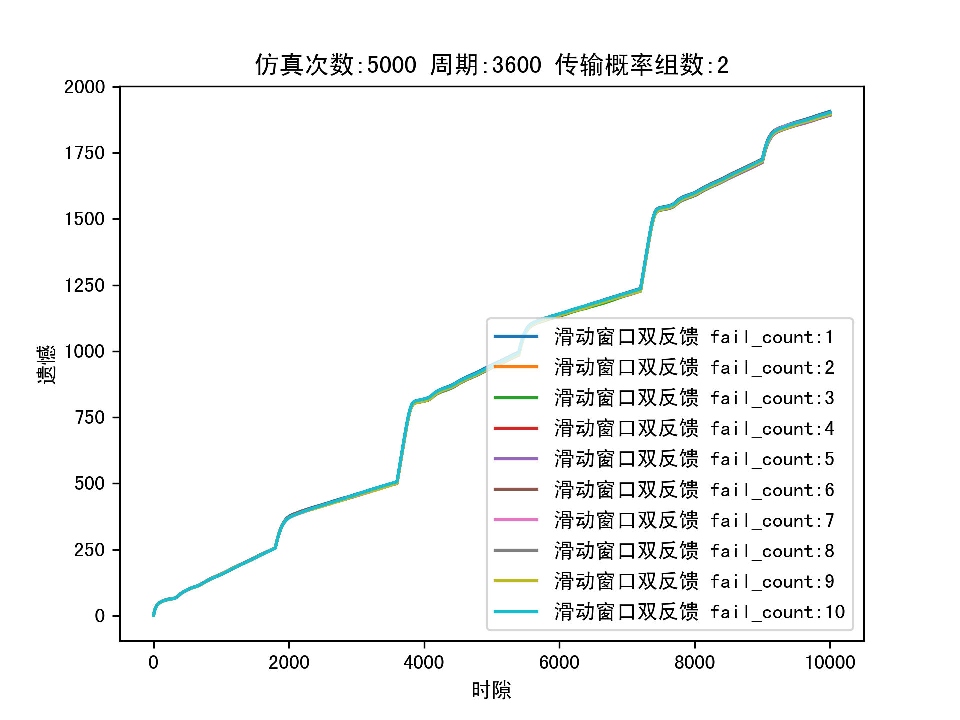
\includegraphics[width=0.8\textwidth]{figure/失败.png}
	\caption{增加失败次数对TS算法的影响}
	\label{fig失败}
\end{figure}

\section{增加成功次数对TS算法的影响}
在这小节,我们选定基于折扣的Thompson Sampling算法来研究折扣系数对TS算法的影响。我们设定了5个折扣系数值,分别为0.1、0.5、0.8、0.9、0.95和1。令人惊讶,图 \ref{fig成功}显示出{增加成功次数到1和2的效果最好。
\begin{figure}[h]
	\centering
	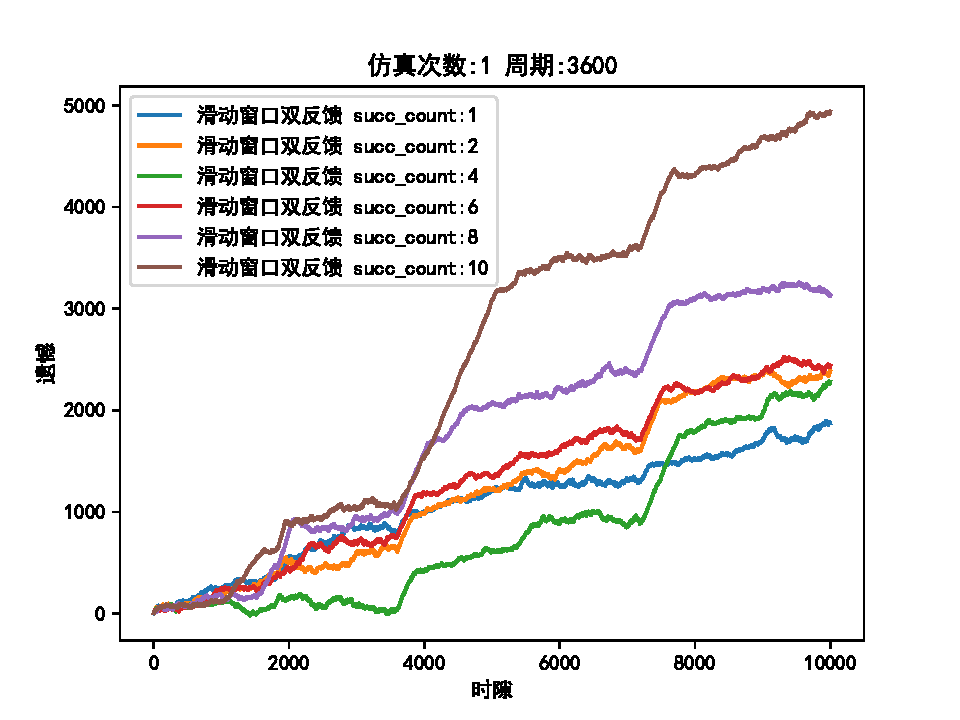
\includegraphics[width=0.8\textwidth]{figure/成功.pdf}
	\caption{增加成功次数对TS算法的影响}
	\label{fig成功}
\end{figure}

\section{折扣滑动窗口TS算法深入探索}
在这一小节,我们深入探索折扣滑动窗口TS算法

\subsection{不同周期下折扣滑动窗口TS算法效果比较}
不同周期对算法的表现还是有很大的影响的,从图 \ref{fig周期}可以看出周期越大,不同周期下折扣滑动窗口TS算法效果越好,这很容易理解,因为周期改变导致TS算法转变所占用的时间变少了。
\begin{figure}[h]
	\centering
	\includegraphics[width=0.8\textwidth]{figure/周期.png}
	\caption{不同周期下折扣滑动窗口TS算法效果比较}
	\label{fig周期}
\end{figure}


\subsection{多种传输概率变换下折扣滑动窗口TS算法效果比较}
我们上面的实验全部都是两组传输概率变换的实验,现在我们使用五十组传输概率来测试折扣滑动窗口TS算法。从图 \ref{fig多概率}可以看出折扣滑动窗口TS算法的表现依然胜过两层反馈TS算法
\begin{figure}[h]
	\centering
	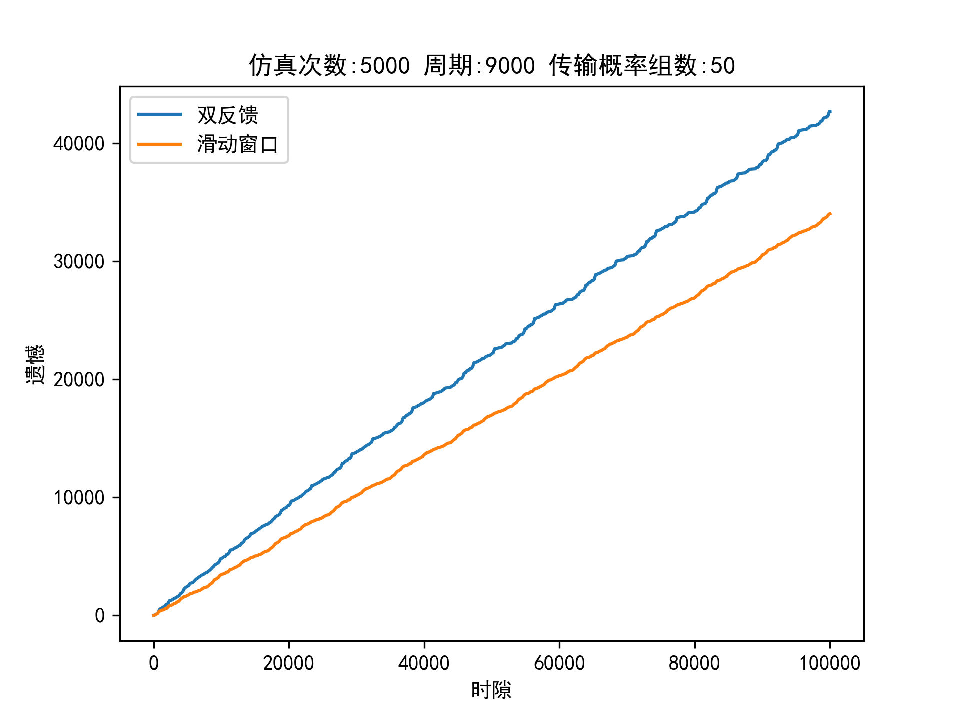
\includegraphics[width=0.8\textwidth]{figure/多概率.png}
	\caption{多种传输概率变换下折扣滑动窗口TS算法效果比较} 
	\label{fig多概率}
\end{figure}

\section{总结}
从上述仿真实验可以看出,我们改进的算法都是非常有效的。

